%%%%%%%%%%%%%%%%%%%MAIN_OPTIONS%%%%%%%%%%%%%%%%%%%
\documentclass[a4paper, 14pt]{article}

%% Работа с русским языком
\usepackage{cmap}					% поиск в PDF
\usepackage{hyperref}				% гиперссылки
\usepackage[warn]{mathtext} 		% русские буквы в формулах
\usepackage[T2A]{fontenc}			% кодировка
\usepackage[utf8]{inputenc}			% кодировка исходного текста
\usepackage[english,russian]{babel}	% локализация и переносы

%% Дополнительная работа с математикой
\usepackage{amsfonts,amssymb,amsthm,mathtools} % AMS
\usepackage{amsmath}
\usepackage{icomma} % "Умная" запятая: $0,2$ --- число, $0, 2$ --- перечисление

%% Номера формул
%\mathtoolsset{showonlyrefs=true} % Показывать номера только у тех формул, на которые есть \eqref{} в тексте.

%%FONTS_Packadges
\usepackage{euscript} % Шрифт Евклид
\usepackage{mathrsfs} % Красивый матшрифт

%% Свои команды
\DeclareMathOperator{\sgn}{\mathop{sgn}}

%% Перенос знаков в формулах (по Львовскому)
\newcommand*{\hm}[1]{#1\nobreak\discretionary{}
	{\hbox{$\mathsurround=0pt #1$}}{}}

%%% Работа с картинками
\usepackage{graphicx}  % Для вставки рисунков
\graphicspath{{pictures/}{images2/}}  % папки с картинками
\setlength\fboxsep{3pt} % Отступ рамки \fbox{} от рисунка
\setlength\fboxrule{1pt} % Толщина линий рамки \fbox{}
\usepackage{wrapfig} % Обтекание рисунков и таблиц текстом
\usepackage[section]{placeins}
\usepackage{subcaption}

%% Работа с таблицами
\usepackage{array,tabularx,tabulary,booktabs} % Дополнительная работа с таблицами
\usepackage{longtable}  % Длинные таблицы
\usepackage{multirow} % Слияние строк в таблице

%%Links
\hypersetup{
	colorlinks=true,
	linkcolor=black,
	filecolor=magenta,      
	urlcolor=blue,
}

%%% Программирование
\usepackage{etoolbox} % логические операторы

%%% Страница
\usepackage{extsizes} % Возможность сделать 14-й шрифт
\usepackage{geometry} % Простой способ задавать поля
\geometry{top=25mm}
\geometry{bottom=35mm}
\geometry{left=20mm}
\geometry{right=20mm}
\usepackage{indentfirst}
%
\usepackage{fancyhdr} % Колонтитулы
\pagestyle{fancy}
\renewcommand{\headrulewidth}{0mm}  % Толщина линейки, отчеркивающей верхний колонтитул
%\lfoot{Нижний левый}
%\rfoot{Нижний правый}
%\rhead{Верхний правый}
%\chead{Верхний в центре}
%\lhead{Верхний левый}
% \cfoot{Нижний в центре} % По умолчанию здесь номер страницы

\usepackage{setspace} % Интерлиньяж
%\onehalfspacing % Интерлиньяж 1.5
%\doublespacing % Интерлиньяж 2
%\singlespacing % Интерлиньяж 1

\usepackage{multicol,caption}

\newenvironment{Figure}
{\par\medskip\noindent\minipage{\linewidth}}
{\endminipage\par\medskip}

\usepackage{enumitem}
\usepackage{amssymb}
\usepackage{xcolor}
%%% Зачеркнутый текст
\usepackage[normalem]{ulem}
\usepackage{xurl}



\begin{document}

	\title{		\textbf{\textit{Победит \#398}} 
		
		Анализ методов сегментации зерен сплава WC-Co}

	\author{$ Д.Г. Каграманян^1, Д.Ю. Камалова^2, Б.Б. Страумал^3, Л.Н. Щур^4$}
	\date{\today}
	\maketitle

	\hfill
	\begin{minipage}{1\textwidth}
			\flushleft
	    $^1$исследователь,dgkagramanyan@edu.hse.ru\\
	    $^2$исследователь,dyukamalova@edu.hse.ru \\
	    $^3$соруководитель,straumal@issp.ac.ru\\
   	 	$^4$руководитель,levshchur@gmail.com\\



	\end{minipage}%

	\section{Аннотация}
	
	Во время решения задачи сегментации зерен сплава WC-Cо возникла неопределенность выбора подхода. 
	Каждый метод показывает свой результат, отличный от других. Неясно какой подход будет оптимален. 

	\section{Задача}
	
	Провести анализ подходов и сравнить какой будет наиболее эффективен при решении задачи сегментации зерен.
	
	\section{Визуальный осмотр}
	
	Визуальный осмотр и анализ исходных фотографий играет важную роль в задачах обработки изображений. 
	
	\subsection{Отсутствие видимых границ}  
	 На изображении микроструктуры отчетливо выделены только границы между зернами и связующим веществом. 
	 Видимые границы между смежными зернами отсутвует, из-за чего возникает сложноотделимая масса из
	  кристаллов сплава (рис. \ref{marked}). 
	 
	 \begin{figure}[h]
	 	\center{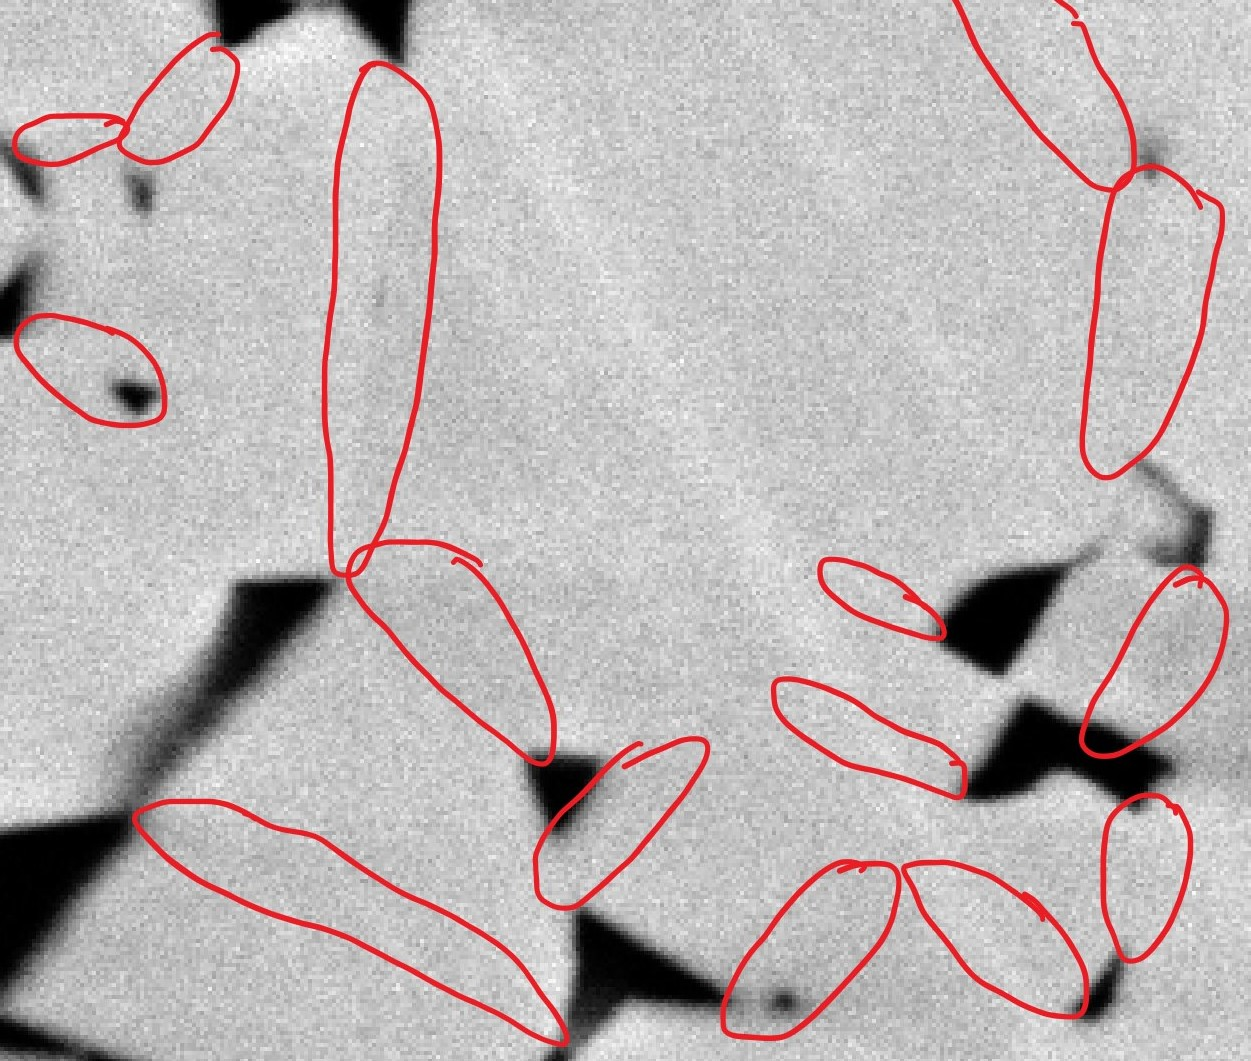
\includegraphics[scale=0.25]{segment_images/grain_zoom_marked}}
	 	\caption{Красными линиями обведены потенциальные границы смежных зерен}
	 	\label{marked}
	 \end{figure}
	 
	 
		
	\subsection{Неравномерное распределение шумов} 
	Большие зерна выделяется на общем фоне уровнем шума, но это неверно для средних и мелких зерен. Если пропустить исходное изображение через детектор границ и контуров \cite{last}, то можно крупные объекты шума можно выделить и соединить их крестиком. Пример такого преобразования  на рисунке \ref{grad_noise_marked} . Их уровень шума примерно на одном уровне.


	 \begin{figure}[h]
			\center{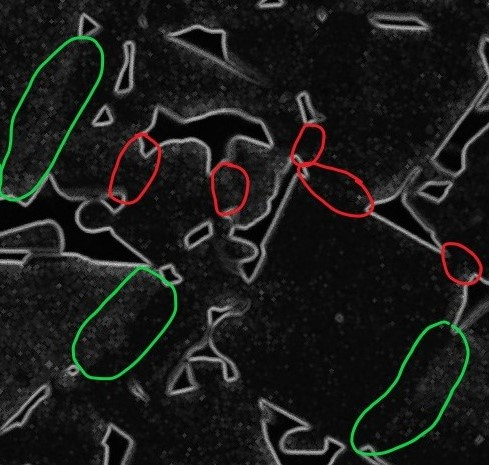
\includegraphics[scale=0.5]{segment_images/grad2_noise_marked}}
			\caption{Зеленой линией отмечено явное изменение шума, обозначающее наличие границы. Красной линией - отсутсвие изменения шума для тех мет, где должна быть гранциа}
			\label{grad_noise_marked}
	\end{figure}


	\section{Возможные подходы решения задачи}
	
	\subsection{Явная сегментация}
	
	Методы сегментации не смогли сегментировать то, чего не видит даже человек
	\subsection{Сегментация на основе шума зерен}
	
	Неточный метод определения границ. Границы больших зерен можно выделить по уровню шума, а средних и мелких - нет
	\subsection{Сегментация на основе EDT}
	
	Euclidean distance transform - преобразование изображения, для которого строится карта расстояний пикселей. 
	
	При первичном осмотре кажется, что указанное преобразование выделяет зерна, но на деле оно создает ту же неразделимую 
	комбинацию зерен (рис. \ref{edt}).
	
	\begin{figure}[h]
		\begin{center}
			\begin{minipage}[h]{0.3\linewidth}
				\center{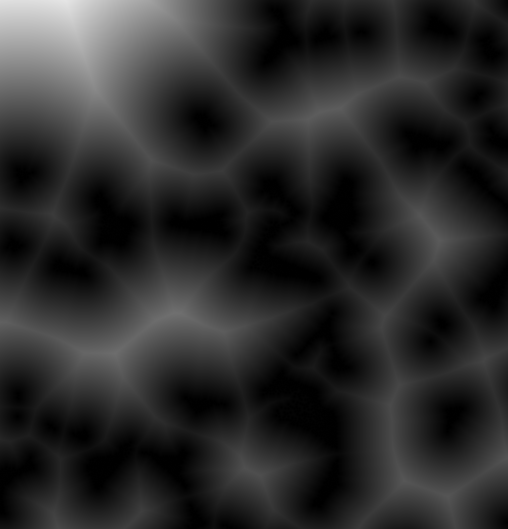
\includegraphics[scale=0.6]{segment_images/dist}}
				\caption{Карта расстояний, полученная преобразованием EDT}
				\label{edt}
			\end{minipage}
			\hfill
			\begin{minipage}[h]{0.5\linewidth}
				\center{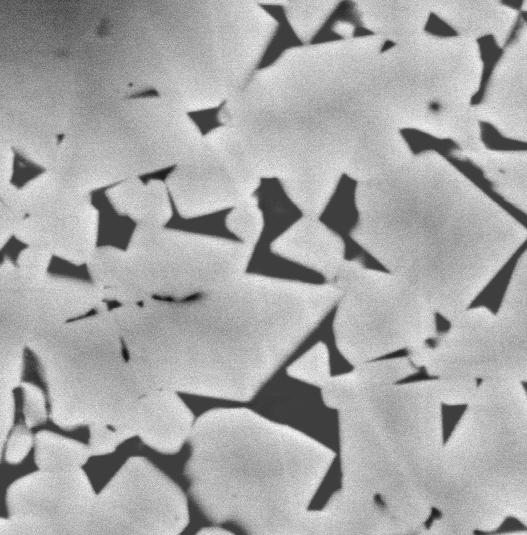
\includegraphics[scale=0.6]{segment_images/dist_inv+image}}
				\caption{Наложение карты расстояний и исходного изображения}
				\label{image+edt}
			\end{minipage}
		\end{center}
	\end{figure}
	
	
	\subsection{Сегментация на основе нейронной сети}
	
	Разметить несколько изображений вручную и подать их на вход нейронной сети.
	Разметка данных -  длительный и монотонный процесс, но благодаря ему можно опустить детали и принцип определения границ пустот. 
	
	Метод имеет место быть, но на деле его применение неоправданно. Затраты времени на разметку слишком большие.  
	
	
	
	
	\subsection{Сегментация на основе контуров пустот}
	\label{final}
	
	Выделим все пустоты и аппроксимируем их контуры с помощью линейной функции (рис. \ref{lines_resized}). Затем будет соединять острые вершины с другими вершинами по особому правилу. По какому - неясно
	
	 \begin{figure}[h]
			\center{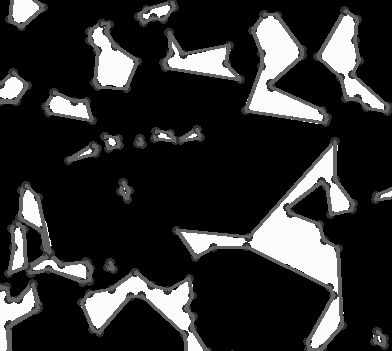
\includegraphics[scale=0.9]{segment_images/lines_resized}}
			\caption{Выделенные пустоты с линейно приближенными контурами}
			\label{lines_resized}
		\end{figure}


\section{Выводы}

Единственный метод, который может показать хороший результат сегментации зерен - графовый алгоритм, проходящий по контурам пустот (глава \ref{final}).

\newpage
%далее сам список используевой литературы
\begin{thebibliography}{}
	
	
	\bibitem{last}  Каграманян Д.Г. -  Cегментации пустот сплава WC-Co
	

		


\end{thebibliography}
	



	
\end{document}